\chapter{协议及其组织结构}

协议是sbid工具中进行建模和验证的有效单元,协议之间是完全相互独立的。

\section{创建协议}
打开sbid工具,点击左上角的[新协议]按钮,或在菜单栏中点击[文件>新协议],即可创建协议面板,如图\ref{create_protocol}所示。
    \begin{figure}[h]
	\centering
	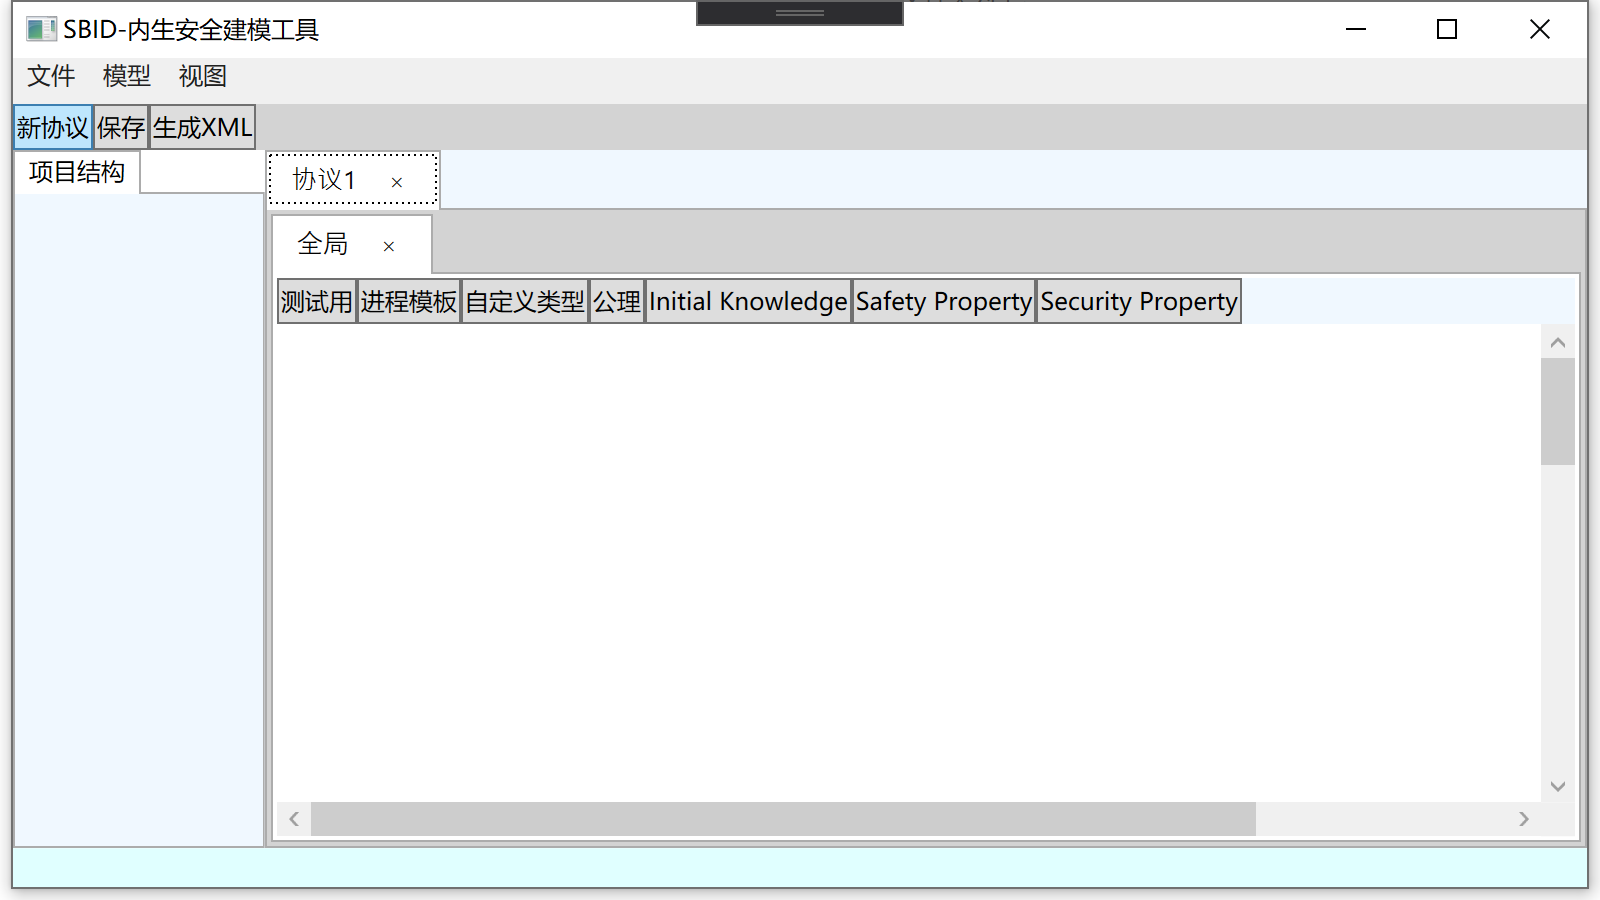
\includegraphics[width=12cm,height=6.75cm]{imgs/create_protocol.png}
	\caption{新创建的协议面板}
	\label{create_protocol}
	\end{figure}
\par
在sbid工具中,可以同时组织多个协议,以便进行协议之间的差异比较。

\section{协议组织结构}
在协议面板下可以组织多个子面板,包括概览(类图)、状态机、攻击树、CTL公式的抽象语法树、顺序图和拓扑图等,如图\ref{protocol_subpanels}所示。
    \begin{figure}[h]
	\centering
	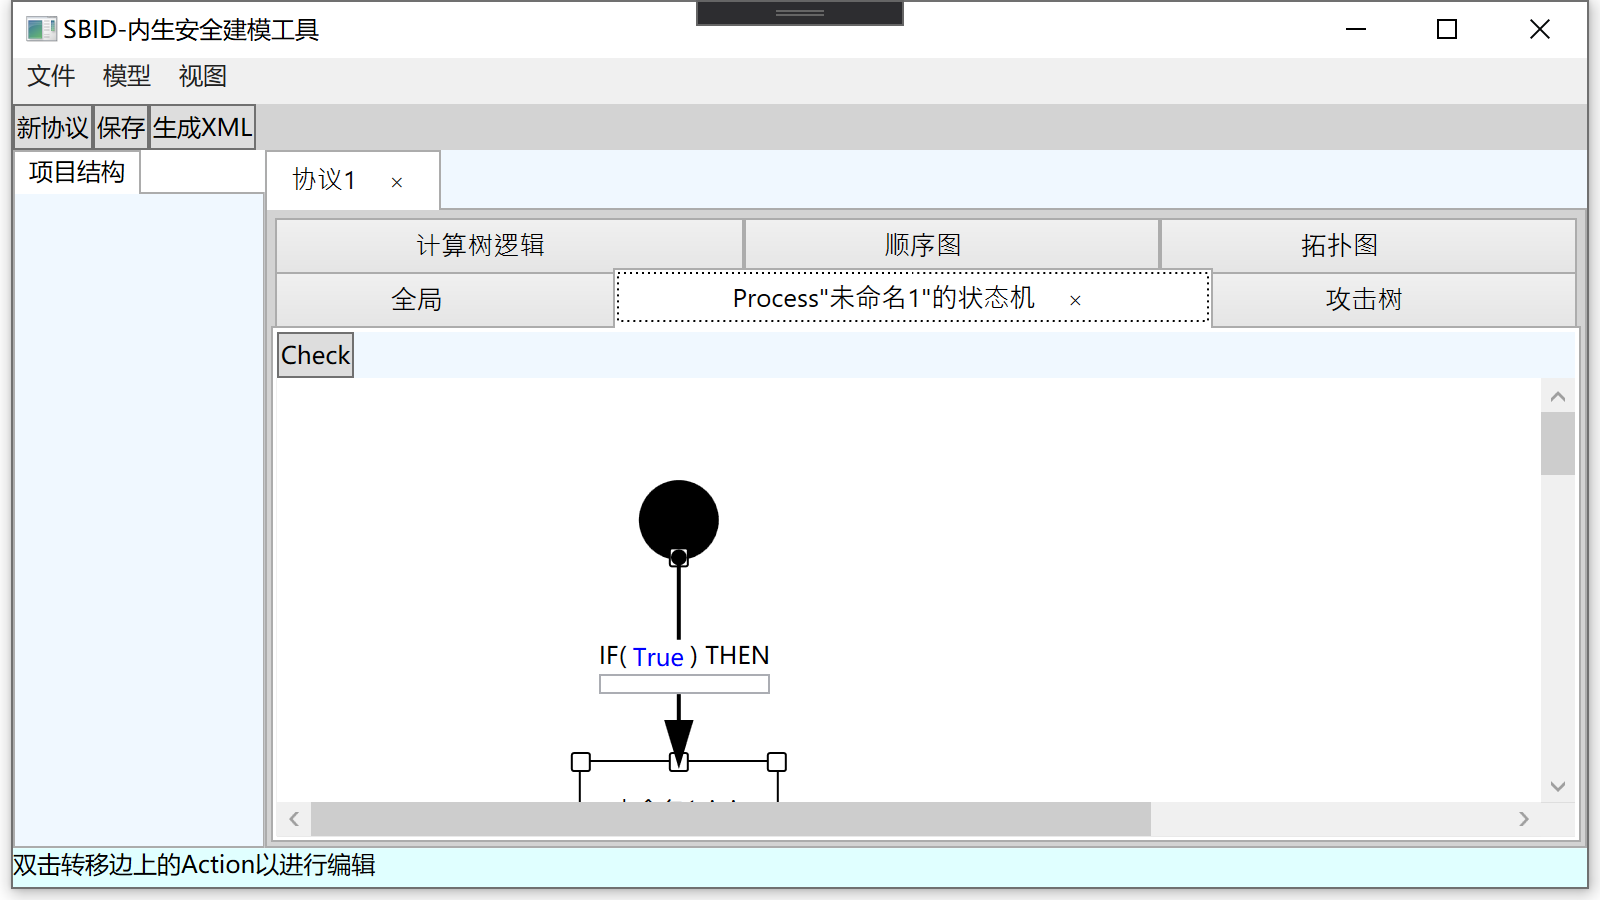
\includegraphics[width=12cm,height=6.75cm]{imgs/protocol_subpanels.png}
	\caption{协议面板的子面板}
	\label{protocol_subpanels}
	\end{figure}